% Author: Marek Fiser <tikz at marekfiser.cz>
% MESIF protocol: http://en.wikipedia.org/wiki/MESIF_protocol
\documentclass[tikz,border=10pt]{standalone}
\usepackage{tikz}
\usetikzlibrary{positioning,shapes,fit,arrows}

%\definecolor{black}{RGB}{56,94,141}
\begin{document}

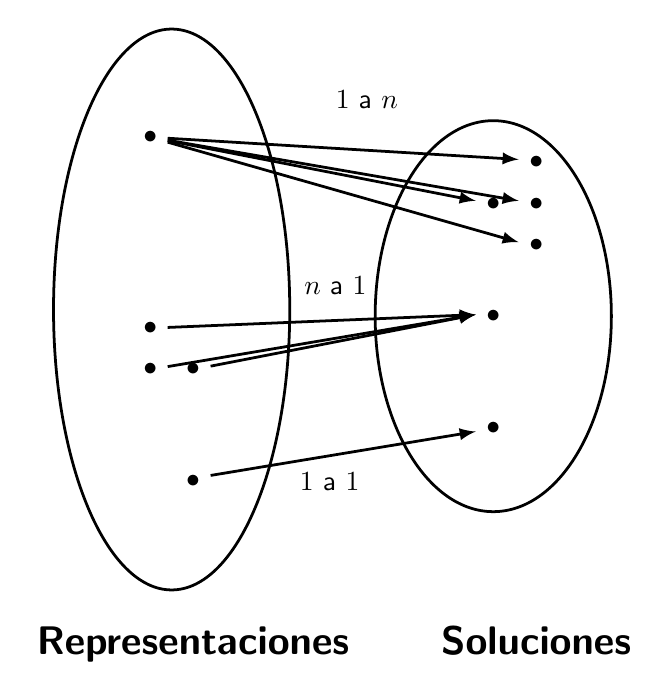
\begin{tikzpicture}[line width=1pt,>=latex]
\sffamily
\node (a1) {$\bullet$};
\node[below= 2cm of a1] (a2) {$\bullet$};
\node[below=.1cm of a2] (a3) {$\bullet$};
\node[right=.1cm of a3] (a4) {$\bullet$};
\node[below=of a4] (a5) {$\bullet$};


\node[right=4cm of a1] (aux1) {};
\node[below= 0.5cm of aux1] (b1) {$\bullet$};
\node[right=0.1cm of b1] (b11){$\bullet$};
\node[above=0.1cm of b11] (b12){$\bullet$};
\node[below=0.1cm of b11] (b13){$\bullet$};
\node[below=of b1] (b2) {$\bullet$};
\node[below=of b2] (b3) {$\bullet$};
\node[right=4cm of a4] (aux2) {};
\node[above right=.02cm and 2cm of a1] (unoan) {$1$ a $n$};
\node[above right=.08cm and 1.6cm of a2] (nauno) {$n$ a $1$};
\node[right= 1cm of a5] (nauno) {$1$ a $1$};
\node[shape=ellipse,draw=black,minimum size=3cm,fit={(a1) (a5)}] {};
    \node[shape=ellipse,draw=black,minimum size=3cm,fit={(b1) (b3)}] {};

\node[below=1.5cm of a5,font=\color{black}\Large\bfseries] {Representaciones};
\node[below=3cm of aux2,font=\color{black}\Large\bfseries] {Soluciones};

\draw[->,black] (a1) -- (b1.170);
\draw[->,black] (a1) -- (b11.170);
\draw[->,black] (a1) -- (b12.170);
\draw[->,black] (a1) -- (b13.170);
\draw[->,black] (a2) --  (b2.175) ;
\draw[->,black] (a3) -- (b2.175);
\draw[->,black] (a4) -- (b2.175);
\draw[->,black] (a5.20) -- (b3.190);
\end{tikzpicture}
\end{document}
